\section{Performance}






Die Tests, die von \cite{shanbhag2014optimizing} bzgl. der Effizienz der Regelmengen durchgeführt wurden, betrachten die Regelmengen RS-B1-CPS, RS-B2 und RS-Graph Rule wobei ein Unterschied zwischen Pellenkoft und Pyro(J) in Abbildung \ref{PellenkoftVsPyro} deutlich wird: Die Regelmenge RS-B1 verwendet Left-Associativity anstatt der Swap Regel. Beide Regeln können mit Hilfe von Kommutativität in einander umgewandelt werden. 
Bei allen Regeln wird die Dauer der Kostenberechnung nicht in die Messung einbezogen. Eine Umwandlung in physische Pläne wurde ebenfalls nicht gemessen.


\begin{figure}[ht]
\centering
\begin{tabular}{|l|l|l|}
\cline{1-3}
{\bf } & {\bf Pellenkoft}                                                                                                  & {\bf Pyro(J)}                                                                                                       \\ \cline{1-3}
{\bf RS-B0-CPS}   & \begin{tabular}[c]{@{}l@{}}Left Associativity\\ Right Associativity\\ Commutativity\end{tabular}            & \begin{tabular}[c]{@{}l@{}}Left Associativity\\ Right Associativity\\ Commutativity\end{tabular}              \\ \cline{1-3}
{\bf RS-B1-CPS }  & \begin{tabular}[c]{@{}l@{}}Swap\\ Bottom Commutativity\end{tabular}                                         & \begin{tabular}[c]{@{}l@{}}Left Associativity\\ Commutativity\end{tabular}                                    \\ \cline{1-3}
{\bf RS-B2 }  & \begin{tabular}[c]{@{}l@{}}Left Associativity\\ Right Associativity\\ Commutativity\\ Exchange\end{tabular} & \begin{tabular}[c]{@{}l@{}}Left Associativity\\ Right Associativity\\ Commutativity\\ Exchange\end{tabular}   \\ \cline{1-3}

{\bf RS-Graph }  &  & \begin{tabular}[c]{@{}l@{}}GraphRule\end{tabular}   \\ \cline{1-3}
\end{tabular}
\caption{Unterschiede zwischen Pellenkoft und Pyro(J)}
\label{PellenkoftVsPyro}
\center
\end{figure}




Die Evaluation testet sowohl kettenförmige, zyklische, sternförmige und kreisförmige Anfragen, wobei die Menge der Relationen variiert. Je mehr Relationen verwendet wurden, desto besser schnitt RS-Graph in den Vergleichstests ab. Die Anfragen, die für die Tests verwendet wurden, beinhalteten nur Join-Operatoren. Aggregation von Relationen wurden daher nicht verwendet.


\begin{figure}[ht]
  \centering
  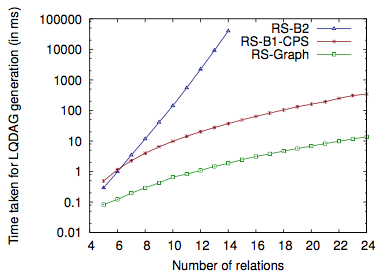
\includegraphics[scale=0.8]{03_Regeln/00_media/Kette.png}
  \caption{Performancechart: Kettenförmige Join-Graphen}
  \label{ketteEval}
\end{figure}

Begonnen wurde mit den kettenförmigen Anfragen. In Abbildung \ref{ketteEval} sind die Ergebnisse zu sehen. Es wurde die Anzahl der Relationen in einer Anfrage immer weiter gesteigert. Eine kettenförmige Anfrage mit $n$ Relationen ist die einfachste Anfrage. Die Regelmenge RS-B2 erreict schnell das absolute Evaluationsmaximum und wird durch den Optimierer abgebrochen. Die Regel RS-B1 ist verglichen mit der neuen GraphRule zu Beginn um den Faktor 10. Der Abstand zwischen RS-B1 und GraphRule vergrößert sich in der Folge immer weiter.

\begin{figure}[ht]
  \centering
  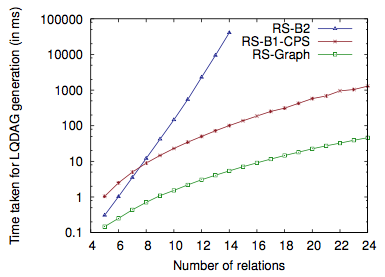
\includegraphics[scale=0.8]{03_Regeln/00_media/cycle.png}
  \caption{Performancechart: zyklische Join-Graphen}
  \label{cycleEval}
\end{figure}

Auch bei der Exploration von Plänen auf Basis eines zyklischen Join-Graphen zeigt sich die Überlegenheit der neuen Regelmenge (vgl. Abb. \ref{cycleEval}).


\begin{figure}[ht]
  \centering
  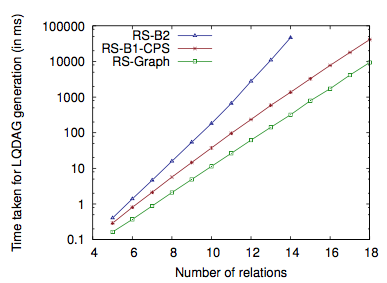
\includegraphics[scale=0.8]{03_Regeln/00_media/star.png}
  \caption{Performancechart: sternförmige Join-Graphen}
  \label{starEval}
\end{figure}

Die Ergebnisse der Messungen für sternförmige Graphen werden in Abb. \ref{starEval} gezeigt.


Die hier gezeigten Ergebnisse dienen als Basis für die in Kapitel 5 vorgestellten eigenen Messergebnisse.


%\subsection{Evaluation}

%Bei der Evaluation der unterschiedlichen Regeln hat sich gezeigt, dass GraphRule eine sehr effektive Regel ist. Sie konnte die beste Performance in allen Vergleichstests erreichen. 

%Bei der Beantwortung der Frage hilft es einen Blick auf die eigentliche Implementierung der GraphRule zu werfen und die Innovation selbst zu betrachten. GraphRule - die genaue Implementierung wurde in Kapitel 3 nachvollzogen - besteht aus einem Interface, dass das Interface der Pyro(J) Regeln erfüllt und einer Implementierung von \texttt{MitCutConservative}. Einiger Code um das Interface mit diesem Algorithmus zu verbinden, war ebenfalls nötig. Wenn man \texttt{MitCutConservative} für sich betrachtet, fällt auf, dass dieser Ansatz in Sachen Performance anderen Verfahren, wie dem Pellenkoft Regelset überlegt ist. Wenn man nun diesem überlegenen Verfahren, das Interface gibt, einer gewöhnlichen Regel in Pyro(J) und alle anderen Regeln entfernt, bleibt dieses Verfahren überlegen. Dieses Ergebnis kann nicht nur intuitiv nachvollzogen, sondern auch durch echte Tests, wie zuvor gesehen, bestätigt werden.





